%%%%%%%%%%%%%%%%%%%%%%%%%%%%%%%%%%%%%%%%%
% Journal Article
% LaTeX Template
% * <feldrandstudios@gmail.com> 2015-01-30T20:40:28.601Z:
%
%
%
% Version 1.3 (9/9/13)
%
% This template has been downloaded from:
% http://www.LaTeXTemplates.com
%
% Original author:
% Frits Wenneker (http://www.howtotex.com)
%
% License:
% CC BY-NC-SA 3.0 (http://creativecommons.org/licenses/by-nc-sa/3.0/)
%
%%%%%%%%%%%%%%%%%%%%%%%%%%%%%%%%%%%%%%%%%

\documentclass[twoside,a4paper]{article}

% --- DOC CONFIG ---

\usepackage[sc]{mathpazo}
\usepackage[T1]{fontenc}
\linespread{1.05}
\usepackage[protrusion=true,expansion=true,final]{microtype}

\usepackage[hmarginratio=1:1,top=32mm,columnsep=20pt]{geometry}
\usepackage{multicol}
\usepackage[hang, small,labelfont=bf,up,textfont=it,up]{caption}
\usepackage{booktabs}
\usepackage{float}
\usepackage{hyperref}
\usepackage{subfigure}

\usepackage{lettrine}
\usepackage{paralist}

\usepackage{abstract}

\usepackage{titlesec}
\titleformat{\section}[block]{\large\scshape\centering}{\thesection.}{1em}{}
\titleformat{\subsection}[block]{\large}{\thesubsection.}{1em}{}

\usepackage{fancyhdr}
\pagestyle{fancy}
\fancyhead{}
\fancyfoot{}
\fancyhead[C]{Selbstorganisierende Karten \(\bullet\) 2014 / 2015 \(\bullet\) ASG Spez.}
\fancyfoot[RO,LE]{\thepage}

\usepackage[english,german]{babel}
\usepackage[utf8]{inputenc}
\usepackage{amsmath,amsthm,amsfonts}
\usepackage{graphicx}
\usepackage[colorinlistoftodos]{todonotes}

\usepackage{minted}

% --- LITTLE TWEAKS ---

\renewcommand{\abstractnamefont}{\normalfont\bfseries}
\renewcommand{\abstracttextfont}{\normalfont\small\itshape}

\renewcommand{\thesection}{\Roman{section}}
\renewcommand{\thesubsection}{\arabic{subsection}}

\newcommand{\haskell}[1]{\mintinline{haskell}|#1|}
\newcommand{\commonlettrine}[1]{\lettrine[nindent=0em,lines=2]{#1}}

% --- DOCUMENT INFORMATION ---

\title{\vspace{-15mm}\fontsize{24pt}{10pt}\selectfont\bfseries{}Buchempfehlungen mit Hilfe von selbstorganisierenden Karten erstellen}

\author{\large\textsc{Julius Quasebarth \quad Luisa Derer \quad Robin Hankel}\thanks{Projektbetreuer: Johannes Suepke, Außenbetreuer: ???}\\[2mm]\normalsize Alber Schweitzer Gymnasium Erfurt (Spez.)\\\vspace{-5mm}}

\date{2014 / 2015}

% --- BEGIN OF DOCUMENT ---

\begin{document}

\maketitle

\thispagestyle{fancy}

% --- BEGIN OF TEXT ---

\begin{otherlanguage}{english}
\begin{abstract}
\noindent
Our super duper cool abstract text...
\end{abstract}
\end{otherlanguage}

\tableofcontents

\section{Einleitung}

\commonlettrine{J}eder kennt das Gefühl der Leere nach dem Lesen eines Buches. Welches Buch soll ich mir als nächstes vornehmen? Ein Buch des selben Autors? Oder doch lieber das Genre entscheiden lassen?
Um das Nachdenken über das nächste Buch kürzer zu machen, haben wir uns dazu entschieden, das Problem im Zuge der Projektarbeit in der 10. Klasse zu lösen.

Dafür nutzen wir selbstorganisierende Karten um Bücher mit dem selben Genre zu empfehlen. Mit diesem mathematischen Prinzip lassen sich Punkte im n-dimensionalem Raum in beliebig viele Gruppen unterteilen, wodurch sich Gruppen von Personen mit ähnlichen Lesevorzügen erstellen lassen. Je nachdem, welche Bücher die Personen bereits gelesen haben, kann somit ein \glqq{}Pool\grqq{} aus Büchern erstellt werden. In unserer Seminarfacharbeit wird vor allem auf die Erstellung des Programms, das Sammeln von Daten dafür und die Anwendung dessen eingegangen.
 
Unsere Ziele sind das Erstellen eines Programmes, welches Bücher mit Hilfe einer selbstorganisierender Karte in viele Gruppen einteilen kann und so Buchempfehlungen ausgibt, das Erklären das Programmes mittels einer schriftlichen Arbeit und das Erstellen einer Internetseite um das Programm nutzbar zu machen.

Um die Funktionsweise des Programmes gut nachvollziehen zu können, werden wir zuerst die Grundlagen einer selbstorganisierenden Karte und neuronaler Netze klären. Im Anschluss werden wir die Wahl unserer Programmiersprache, Haskell, begründen. Als nächstes folgt die Erklärung der mathematischen Prinzipien welche wir für unser Programm nutzen. Die Erklärung des Programms schließt sich an, wobei erst die wichtigsten Funktionen behandelt und dann auf die Nebenfunktionen eingegangen wird. Der folgende Abschnitt beschreibt die Anwendungen, für die unser Programm genutzt werden kann. Dabei wird vor allem Wert auf die Kundenempfehlung im Onlinehanedel gelegt. Auch Anwendungen, welche schon genutzt werden, werden erkärt. Abschließen wird die Arbeit mit dem Beschreiben unserer Internetseite.

\section{Mathematische Prinzipien der selbstorganisierenden Karte}
\subsection{Neuronale Netze --- Grundlagen für ein besseres Verständnis}

\commonlettrine{D}ie selbstorganisierende Karte ist vom Prinzip her ein neuronales Netz, welches, anders als \glqq{}normale\grqq{} neuronale Netze (wie z.B. das Backpropagation-Netz), unüberwacht lernt und deren Ergebnisse stark von der Anordnung der Neuronen abhängig sind. Doch was bedeutet das überhaupt? Was ist ein neuronales Netzwerk, was heißt \glqq{}unüberwacht\grqq{} und warum sind die Ausgaben des Netzwerkes von der Anordnung der Neuronen abhängig?

Ein neuronales Netzwerk ist ein Netzwerk aus Neuronen, das heißt, die Neuronen sind miteinander über sogenannte Synapsen bzw. Gewichte verbunden (diese Begriffe werden Synonym verwendet). Die Synapsen verbinden die Ausgänge der Neuronen mit den Eingängen (meist) anderer Neuronen (es können manchmal auch Verbindungen von einem Neuron zu demselben vorhanden sein). Sie übertragen Daten, diese sind normalerweise rationale Zahlen (also Zahlen, die sich als Bruch darstellen lassen). Ein Neuron erhält nun folgende Eingaben: Die Daten, die andere Neuronen über die Synapsen zu ihm schicken, und die \glqq{}Gewichte\grqq{} dieser Synapsen --- dies sind Konstanten, die jeder Synapse zugeordnet werden können. Mit speziellen Funktionen kann das Neuron nun diese Daten verarbeiten und zu einem Wert kombinieren (mit Hilfe einer sogenannten Propagierungsfunktion), den es dann über seine Ausgabesynapsen ausgibt (dieser Wert wird durch die Aktivierungsfunktion berechnet). Da ein neuronales Netzwerk noch Eingaben von außen benötigt, um jene Eingaben zu verarbeiten, existieren Spezialfälle: So gibt es Eingabeneuronen, die lediglich das ausgeben (oder \glqq{}feuern\grqq{}), was man selbst bestimmt, ebenso wie Ausgabeneuronen, die ihre Ausgaben nicht wieder in das neuronale Netz einspeisen, sondern in die reale Welt ausgeben.

Das Besondere an neuronalen Netzen ist, dass diese lernen können. Dazu gibt es spezielle Algorithmen, wie etwa den Backpropagation-Algorithmus: Dabei wird versucht, herauszufinden, wie man das neuronale Netz verbessern kann, indem man bestimmt, welches Neuron welchen \emph{Fehler} im neuronalen Netz verursacht hat. Man speist Eingaben, zu denen man die optimalen Ausgaben kennt, in das neuronale Netz ein und vergleicht die Ausgaben des neuronalen Netzes mit den erwarteten Ausgaben. Danach kann man bestimmen, welches Neuron wie stark zu dem Unterschied zwischen gewünschten und tatsächlichen Ausgaben beigetragen hat und darauf basierend die Gewichte zwischen den Neuronen ändern. Da das neuronale Netz bei diesem Algorithmus nach einem vorgegebenem Ausgabemuster trainiert wird, lernt das Netz \glqq{}überwacht\grqq{}.

Im Gegenteil dazu steht das unüberwachte Lernen. Dabei geht es oft darum, Daten zu gruppieren und einzuordnen. Zum Beispiel kann ein neuronales Netz, das unüberwacht lernt, mit den Bildern von Buchstaben trainiert werden und anschließend andere Bilder in diese Buchstabengruppen einsortieren.

\subsection{Die selbstorganisierende Karte im Vergleich zu anderen neuronalen Netzwerken}

\commonlettrine{D}ie selbstorganisierende Karte, eine besondere Form eines neuronalen Netzes, lernt auch unüberwacht. Sie ist aus zwei Schichten von Neuronen aufgebaut, das heißt, jedes Neuron aus einer Schicht ist mit jedem Neuron aus einer anderen Schicht verbunden, jedoch sind die Neuronen aus einer Schicht untereinander nicht verbunden. Die erste Schicht, Eingabeschicht genannt, ist besetzt mit \(n\) Eingabeneuronen, wobei \(n\) die Anzahl von Dimensionen ist, die die zu gruppierenden Punkte haben sollen. Die zweite Schicht, Kohonenkarte genannt, besteht aus Neuronen, die die Gruppen repräsentieren; Die Gewichte von jedem Eingabeneuron zu einem Neuron \(k\) aus der Kohonenkarte sind dabei als Koordinaten im Raum zu verstehen. Alle Punkte, die näher an dieser Koordinate sind als an Koordinaten anderer Punkte, gehören zur Gruppe \(k\)s. Wenn die Propagierungsfunktion eines jeden Neurons aus der Kohonenkarte also
\[
\sqrt{\sum_{i\in{}E} \left((w_{i\rightarrow{}k} - v_i)^2\right)}
\]
lautet\footnote{Diese Funktion spiegelt letztendlich den euklidischen Abstand von dem eingegebenem Punkt zum Repräsentationspunkt des betrachteten Neurons aus der Kohonenschicht wider.} (wobei \(w_{i\rightarrow{}j}\) das Gewicht von Neuron \(i\) zu Neuron \(j\), \(v_i\) die Ausgabe des Neurons \(i\) und \(E\) die Menge der Eingabeneuronen bezeichnet), dann gehört der Punkt, der durch die Eingabeneuronen definiert wurde, zu dem Neuron aus der Kohonenschicht, welches den geringsten Ausgabewert hat (dieses soll mit \glqq{}Gewinnerneuron\grqq{} bezeichnet werden).

Die selbstorganisierende Karte lernt, indem der Repräsentationspunkt eines Neurons der Kohonenkarte verschoben wird. Dazu gibt man ein Eingabemuster in das Netz ein und verschiebt den Repräsentationspunkt des Gewinnerneurons um einen bestimmten Anteil in Richtung des eingegebenen Punktes. Interessant hierbei ist, dass auch Neuronen in der unmittelbaren Umgebung des Gewinnerneurons in Richtung des eingegebenen Punktes verschoben werden können: Somit können sich die Repräsentationspunkte im Raum auf ähnliche Weise anordnen, wie die Neuronen der Kohonenschicht angeordnet sind.

\subsection{Anwendung der Prinzipien der selbstorganisierenden Karte}

Natürlich finden die oben beschriebenen Prinzipien auch in der Praxis Anwendung. Besonders, wenn Informationen vorverarbeitet werden müssen, wenn milliarden Datenpunkte zu wenigen tausend umgewandelt werden sollen, sind selbstorganisierende Karten von Bedeutung. Sie gruppieren Daten, um Auffälligkeiten und Muster in der Verteilung dieser aufzudecken. Weil selbstorganisierende Karten jedoch so viele Daten verarbeiten müssen, lohnt es sich auch, diese besonders effizient zu gestalten. Wie kann man also eine selbstorganisierende Karte simulieren, ohne unnötige Rechenzeit zu verbrauchen?

Das wichtigste Stichwort zur Antwort auf diese Frage ist Minimalismus. Unnötige Konstruktionen werden nicht gebraucht, also auch nicht umgesetzt. Daher muss man überlegen, welche Teile der Grundlagen vereinfachbar sind und welche nicht. Zum Beispiel muss man nicht jeden Prototypen als Neuron mit Propagierungs- und Aktivierungsfunktion sehen (da diese ja bei allen Prototypen gleich sind), man muss also nicht einmal ein Netz dieser simulieren. Was ist dann besonders wichtig für die selbstorganisierende Karte?

\begin{enumerate}
\item Prototypen. Die wichtigsten Informationen, die diese tragen, sind ihre Repräsentationspunkte im mehrdimensionalen Raum und ihre Position im Prototypenraum (also in der Kohonenkarte). Die Datenpunkte, mit denen die Prototypen eine Gruppe bilden, müssen nicht explizit in Verbindung mit den Prototypen gebracht werden, da man diese Verbindung auch nachträglich noch ausrechnen kann.

\item Die Datenpunkte, da diese natürlich die wichtigsten Informationen enthalten. Sie tragen genauso wie die Prototypen eine Koordinate im mehrdimensionalen Raum.

\item Eine \(\alpha\)-Funktion (bzw. Alphafunktion). Diese wird benötigt, um klarzustellen, wie stark die Prototypen durch die Datenpunkte beeinflusst werden können. Sie nimmt die Position des Gewinnerprototypen entgegen und ordnet dann jedem Prototypen die beeinflussbarkeit dessen zu.
\end{enumerate}

Wie zu erkennen ist, ist die selbstorganisierende Karte im Wesen nicht sonderlich kompliziert. Mit wenigen Grundlagen kann man sie also realisieren.

\section{Erklärung und Vorstellung des Programms}

\subsection{Begründung der Wahl der Programmiersprache}

Unser Programm, um welches es in dieser Arbeit geht, ist in Haskell geschrieben. Haskell ist eine funktionale Programmiersprache und somit sehr anders aufgebaut als imperative, objektorientierte Programmiersprachen. Funktionalität bedeutet:

\begin{enumerate}
\item Keine Variable darf verändert werden. Dies ist einer der Grundsätze der funktionalen Programmierung, denn durch dieses Prinzip ist es formal egal, in welcher Reihenfolge Prozesse ausgeführt werden.

\item Eine Funktion gibt bei gleichen Parametern gleiche Ausgaben aus. Mit anderen Worten sind (die meisten) Funktionen in Haskell daher \glqq{}pure\grqq{} und verursachen keine \glqq{}side-effects\grqq{}, interagieren also nicht mit der Außenwelt.
\end{enumerate}

Dadurch entstehen allerdings Probleme bei In- und Output: Jede Funktion, die z.B. Eingaben vom Nutzer verarbeitet, ist \glqq{}impure\grqq{} (unrein), da ihre Ausgaben nicht nur von ihrer Parameterliste, sondern auch von der Außenwelt (dem Nutzer) abhängig sind. Haskell löst dieses Problem, indem jede Funktion, die Kontakt zur Außenwelt aufnimmt, markiert wird. Dies geschieht, indem Daten, die aus der Außenwelt stammen, in einem sogenanntem \glqq{}Monad\grqq{} verkapselt werden. Ein Monad ist eine Datenstruktur, deren Daten zwar weiter verarbeitet, aber nicht unbedingt aus dem Monad extrahiert werden können. Somit werden Daten, die durch In- und Output verursacht wurden (da es in Haskell keine Funktionen gibt, die nichts zurückgeben, da dies sinnlos wäre, geben auch Ausgabefunktionen etwas zurück) immer in einem \glqq{}IO-Monad\grqq{} gespeichert und können nicht wieder aus diesem extrahiert werden. Daher kann einfach bestimmt werden, ob eine Funktion mit der Außenwelt kommuniziert, indem die Typsignatur (besonders die Rückgabe der Funktion) beobachtet wird.

Des weiteren verfolgt Haskell die Philosophie der \glqq{}lazy evaluation\grqq{}, wodurch Variablen erst dann ausgewertet werden, wenn sie auch benötigt werden (z.B. wenn eine Variable ausgegeben werden muss). Dadurch wird Rechenzeit gespart, da unbenötigte Ergebnisse auch nicht berechnet werden. Auch gibt es eine effiziente Umsetzung von Rekursivität in Haskell, was viele Funktionen vereinfacht und eleganter macht. Schließlich kompiliert der Haskell Compiler (in dieser Seminarfacharbeit wurde der am weitesten verbreitete Glasglow Haskell Compiler, oder GHC, verwendet) den Quellcode direkt in Assemblercode, wodurch, anders als bei Java, das Programm maschinenfreundlich --- und damit schneller --- ausgeführt wird.

Für unser Programm brachten diese Umstände vor allem folgende Vorteile:

\begin{enumerate}
\item Die Schnelligkeit, die Haskell mit sich bringt, ist äußerst bedeutend. Weil eine selbstorganisierende Karte viele Daten verarbeiten muss, ist dieser Faktor nicht zu vernachlässigen.

\item Haskell ist eine Programmiersprache, die sich in äußerst kurzer und prägnanter Form schreiben lässt. Dadurch ist es oftmals einfacher, den Überblick über ein in Haskell geschriebenes Programm zu behalten --- es bedeutet jedoch nicht, dass es einfacher ist, Programme in Haskell zu schreiben, denn es ist eine höhere Konzentration zum Schreiben dieser benötigt.

\item Viele Datenstrukturen in Haskell sind wiederverwendbar: In den meisten objektorientierten Programmiersprachen trifft dies nicht zu. Stattdessen wird in jenen jede Datenstruktur für einen bestimmten Zweck verwendet, während Haskell darauf aufbaut, Datenstrukturen so abstrakt wie möglich zu halten.

\item Haskells eigenes \glqq{}build system\grqq{}, cabal, ist in der Haskell Plattform erreichbar. Somit wird es für den Programmierer einfacher, Bibliotheken von Anderen (welche in großer Qualität und Zahl vorhanden sind) in das eigene Programm einzubinden.

\item Schließlich läuft Haskell auch auf den meisten Betriebssystemen (Windows, Linux, OSX, \dots{}); Da es jedoch nicht nur einen Compiler gibt und die Sprache Haskell letztendlich nur eine Konvention ist, kann sie auch nach Bedarf auf andere Betriebssysteme übertragen werden.
\end{enumerate}

\subsection{Das Programm \glqq{}SOMC.hs\grqq{}}

Das Wissen über selbstorganisierende Karten wurde in einem Programm umgesetzt, welches aus historischen Gründen den Namen SOMC.hs trägt. Die API-Dokumentation ist auf englisch unter \url{sammex.github.io/project-som/SOMC.html} erhältlich. Weil es nicht von Nutzen wäre, diese hier zu wiederholen, soll hauptsächlich auf die Ideen und Funktionsweisen des Programmes eingegangen werden.

Am wichtigsten ist ganz eindeutig die Funktion \haskell{epoch}, da diese eine Iteration über eine selbstorganisierende Karte tätigt: Dabei wird für jeden Datenpunkt der näheste Prototyp bestimmt (siehe \haskell{getWinner}) und dann darauf basierend die Prototypen aktualisiert (siehe \haskell{updateWinner}). Die \haskell{epoch}-Funktion ist ein grundlegender, wenn auch nicht komplexer Baustein für das Programm. Die \haskell{train}-Funktion ist auf ihr aufgebaut; Diese wiederholt \haskell{epoch} immer wieder. Dabei sollen sich allerdings die \(\alpha\)-Werte ändern, weil die Prototypen zu den beginnenden Iterationen sehr stark verschoben werden sollen, um sich gleichmäßig zu verteilen, aber später weniger, damit sie akkurate Gruppen bilden. Insgesamt ist es sinnvoll, verschiedene Werte über die Iterationen zu verändern: So z.B. den Radius, in dem die Prototypen aktualisiert werden; Oder der \(\alpha\)-Wert über die verschiedenen Radii: Prototypen, welche im Prototypenraum in einem bestimmten Abstand zueinander sind, sollen auch angemessen verschoben werden, wenn einer der beiden am nächsten zu einem Datenpunkt ist. Um sowohl die Bibliothek im Programm benutzerfreundlicher zu machen und Boilerplate-Code zu reduzieren, haben wir deshalb folgenden Ansatz an das Problem der Konfiguration verschiedener Verteilungen gewählt: Die Paradigmen der funktionalen Programmierung. Das bedeutet in diesem Sinne, dass Funktionen miteinander kombiniert werden. So konnten wir ein Gerüst schaffen:

\begin{enumerate}
\item Alpha-Funktionen sind diejenigen Funktionen, in die alle darauf folgenden eingespeist werden. Sie selbst beschreiben den Verlauf des Gewinner-Alphas über die Iterationen, was bedeuten soll, dass sie \emph{Richtwerte} für später aufgerufene Funktionen liefern. Betrachten wir als Beispiel \haskell{quadraticAlpha}: Als Argumente nimmt es --- neben den ersten beiden Argumenten, welche in den nächsten Punkten geklärt werden --- einen Anfangs-Alpha-Wert entgegen, dann die Anzahl der Trainingsdurchläufe, die die selbstorganisierende Karte erfahren wird, dann die Nummer des aktuellen Trainingsdurchlaufes (\emph{da die \haskell{quadraticAlpha} in \haskell{train} aufgerufen wird (!)}) und schließlich die Position des gewinnenden Prototyps in einer Iteration und die Position eines Prototyps, dessen Alpha- bzw. Verschiebungswert berechnet werden soll.

\begin{figure}
\centering
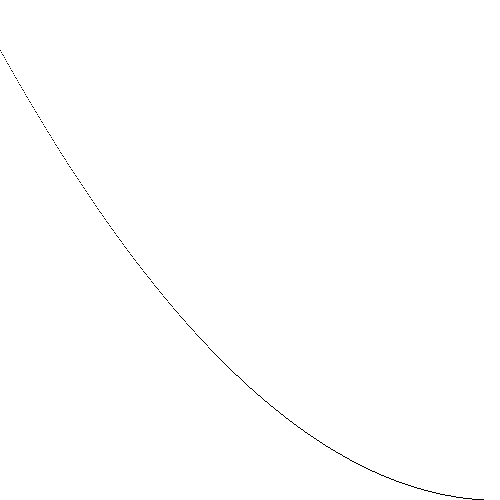
\includegraphics[width=0.4\textwidth]{src/quadAlph.png}
\caption{Der Verlauf der quadraticAlpha-Funktion über Iterationen.}
\end{figure}

\item Das erste Argument einer \haskell{...Alpha}-Funktion ist die Verteilung des Radius' über Iterationen: Man beachte dabei den Typ \haskell{Int -> Int ->}, welcher sowohl in der Typsignatur des Arguments als auch in der der \haskell{...Alpha}-Funktion vorkommt; Tatsächlich hat dieser immer die gleiche Bedeutung, nämlich \haskell{Anzahl der Iteration -> Aktuelle Iteration -> Int}. Dabei ist der Rückgabewert gleich dem Radius, der in der aktuellen Iteration verwendet werden soll.

\begin{figure}
\centering

\includegraphics[width=0.4\textwidth]{src/sqRad.png}
\caption{Der Radius, welcher von der \haskell{squareRadius}-Funktion generiert wird, in Abhängigkeit von den Iterationen.}
\end{figure}

\item Das zweite Argument einer \haskell{...Alpha}-Funktion ist vom Typ \haskell{Int -> Double -> Vec Int ->} \haskell{Vec Int -> Double}, was gleichzusetzen ist mit \haskell{Radius -> Alpha In Der Iteration ->} \haskell{Gewinner-Prototyp-Position ->} \haskell{Zu Verschiebender Prototyp -> Alpha-Wert}. Grundstein dieser Funktion ist eine Interpretation des Prototypenraums, d.h., eine Funktion, welche den Koordinaten von zwei Prototypen einen Radius zuordnen kann. Ein Beispiel hierfür ist die \haskell{squareInterpretation}, welche die Verteilung der Prototypen auf klassischen quadratischen Teilen annimmt, aber auch andere Interpretationen wie etwa eine hexagonale, bei der Prototypen auch versetzt dargestestellt werden, sind möglich.

\item Damit eine Interpretation des Prototypenraumes komplett ist, benötigt sie Informationen darüber, wie sich das Alpha verändern soll, wenn der Abstand von einem Prototyp zum Gewinner größer wird. Diese Information wird von Funktionen wie der \haskell{squareRadiusDistribution} gegeben; Dabei sind die Argumente dieser der Alpha-Wert des Gewinner-Prototypen, der maximal mögliche Radius zum Gewinner-Prototypen, bei dem ein Prototyp trotzdem noch verschoben wird, und der Abstand vom momentan zu verschiebendem Prototyp zum Gewinner-Prototyp. Die \haskell{squareRadiusDistribution} an sich verfolgt ein äquivalentes Muster wie \haskell{squareRadius} und \haskell{quadraticAlpha}; Tatsächlich sind die genutzten Gleichung identisch.

\begin{figure}
\centering
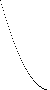
\includegraphics[width=0.4\textwidth,height=0.2\textheight,keepaspectratio]{src/sqRadDistr.png}
\caption{Der Verlauf des Alpha-Werts bei größerem Abstand zum Gewinner-Prototyp mit der \haskell{squareRadiusDistribution}.}
\end{figure}
\end{enumerate}

Wendet man diese Funktionen nun an, so kann sich als Argument für \haskell{train} nun etwas ergeben wie etwa \haskell{reversedAlpha (squareRadius 3)} \haskell{(squareInterpretation} \haskell{squareRadiusDistribution)} \haskell{0.3}. Nach kurzem Nachdenken sollte klar werden, wie dies zu interpretieren ist.

Wir erweiterten unser Programm um eine graphische Seite, deren Funktionen zwar nicht erklärenswert, deren Ausgaben allerdings interessant für den Beweis der Funktion selbstorganisierender Karten sind. Abgesehen von den Alpha-Funktionen wurde dazu immer die bereits oben kreierte genutzt, in 100 Trainingsdurchläufen.

\begin{figure}
\centering
\subfigure[Gruppierung mit \haskell{linearAlpha}]{
	
\includegraphics[width=0.3\textwidth]{src/TestL/origMDCSGroups.png}
	
\includegraphics[width=0.3\textwidth]{src/TestL/finalMDCSGroups.png}
}
\subfigure[Gruppierung mit \haskell{quadraticAlpha}]{
	
\includegraphics[width=0.3\textwidth]{src/TestQ/origMDCSGroups.png}
	
\includegraphics[width=0.3\textwidth]{src/TestQ/finalMDCSGroups.png}
}
\subfigure[Gruppierung mit \haskell{reversedAlpha}]{
	
\includegraphics[width=0.3\textwidth]{src/TestR/origMDCSGroups.png}
	
\includegraphics[width=0.3\textwidth]{src/TestR/finalMDCSGroups.png}
}
\caption{Verschiedene Gruppierungen zufällig generierter Daten. Jeweils links: Vor der Anwendung, rechts: Danach; Man beachte die Gruppen, die anfangs sehr klein bzw. ungleichmäßig verteilt sind und später durch die selbstorganisierende Karte ausgeweitet wurden, oder auch die neue Farbanordnung.}
\end{figure}

\section{Anwendug neuronaler Netze}

\subsection{Individuelle Produktempfehlungen als Verkaufsförderndes Prinzip im Online-Handel}

Mit der heutigen zunehmenden Verlagerung der Kaufumgebung in die digitale Welt des Online-Handels steigt auch der Bedarf nach individualisierter Kundenberatung und Ausgestaltung der Online-Shops. Die spezielle Anpassung an den einzelnen Besucher dient damit als eine verkaufsfördernde Maßnahme, die bereits bei einem großen Teil der Händler Anwendung findet.

Online-Shops dienen allein dazu, den Verkaufsumsatz eines Händlers weiter zu steigern. Diese Art des Shoppings ist für den Kunden die angenehmste, da er zum Erwerb des gesuchten Produktes nicht einen Laden aufsuchen muss, sondern es bequem von Zuhause aus bestellen kann. Außerdem ist das Sortiment eines Verkäufers so schneller einsehbar, was eventuelle Kaufwege für den Kunden erleichtern und verkürzen kann. Es existieren also für den Verbraucher genug Gründe, Online-Shops zu nutzen. Die Online-Branche boomt durch die neue Nachfrage und immer mehr Händler steigen, der Erfolgsaussicht wegen, auf diese Art der Vermarktung um.

Es ist jedoch wichtig für die Anbieter, den Erfolg eines Online-Shops kalkulieren und damit kontrollieren zu können. Die dafür nötige Erfolgsmessung besteht aus zwei Hauptkomponenten: Dem Traffic, welcher die Anzahl und Verweildauer der Besucher beschreibt, und die Conversion-Rate, die die Umwandlung von Besuchern bzw. Interessenten in Kunden angibt. Zur höchstmöglichen Optimierung dieser Faktoren gibt es viele verschiedene Strategien und Prinzipien, wie beispielsweise Qualitätssiegel oder Kundenbewertungen. Diese sollen den Besucher dazu bringen, sein Vertrauen in die Seriosität des Shops und die Qualität der Produkte zu steigern und ihn so zu einem aktiven Kunden zu machen.

Eine sehr gebräuchliche und allgemein meistens genutzte Methode, um dies zu erreichen, sind Kundenberatungen. Ein Kundenberater kennt den Landen und die Produkte genau und kann sich auf den individuellen Kunden einstellen. Doch dies funktioniert nicht nur in begehbaren Geschäften, sondern ist auch mittlerweile in Online-Shops möglich. Produktempfehlungssysteme dienen dort dem (potenziellen) Kunden als virtueller Kaufberater, der bei der Auswahl der Produkte behilflich sein kann. Die gebotenen Empfehlungen werden dadurch optimiert, dass das System das Verhalten des Kunden lernt und so bessere Vorhersagen über dessen Geschmack treffen kann. Zusätzlich analysiert es das Verhalten der anderen Kunden,  kann Parallelen zwischen den Interessen und dem Verhalten erkennen und die damit verbundenen Erfahrungen in die Kaufberatung einfließen lassen (siehe Kapitel 5.3, „Datenanalyse“). Da dies in Echtzeit geschieht, wird die Wirkung der Empfehlungen verbessert und der Warenkorb vergrößert.

Als Fazit lässt sich sagen, dass Empfehlungssysteme ein sehr effektives Vermarktungsmittel in Online-Shops darstellen. Sie wirken sich vermutlich am meisten auf die Wahrnehmung und damit die Kaufentscheidung der Kunden aus, da die individuell auf das Verhalten des Kunden abgestimmten Empfehlungen und die Anpassungsfähigkeit in Echtzeit von dem Kunden als besonders hilfreich angesehen werden. Damit wirkt sich das Verfahren auch positiv auf die Größe des Warenkorbes des Käufers aus.

\subsection{Weitere Anwendungsmöglichkeiten neuronaler Netze}

\subsubsection{Mustererkennung}

Die Mustererkennung ist ein sehr vielfältiger sowie anspruchsvoller Bereich für die Anwendung von künstlichen neuronalen Netzen, der uns nicht nur im Alltag häufig begegnet. Ein Teilbereich dessen ist beispielsweise die automatische Gesichtserkennung. Der komplexe neurologische Vorgang, sich das Gesicht anderer Personen merken und wiedererkennen  zu können, begleitet uns schon von klein auf durch den Alltag und erscheint ganz selbstverständlich. Doch mittlerweile wird diese Fähigkeit auch in der Computerbranche verlangt und kann mithilfe von künstlichen neuronalen Netzen verwirklicht werden. Sie werden eingesetzt um unterschiedliche Ansichten eines Gesichts zu verknüpfen und einer bestimmten Person zuzuordnen, um dann durch Selbstorganisation Klassen zu bilden. Fehlertoleranz und Generalisierungsfähigkeit sind dabei enorm wichtig, da Ausrichtung, Position oder Beleuchtung des Gesichts variieren können. Doch nicht nur die Gesichtserkennung sondern zum Beispiel auch Fingerabdruck-, Handschrift- und Spracherkennung finden schon in modernen Smartphones Anwendung.

Eine weitere Anwendungsmöglichkeit findet die Mustererkennung in der Medizin. Dort dient sie als Unterstützung in der Diagnostik oder der Interpretation von EKG, EEG, Röntgen-, Ultraschall- oder Computertomographiebildern.

\subsubsection{Prognosen}

Um wirtschaftliche Prognosen stellen zu können ist es notwendig, ein Modell eines Bereiches zu erstellen um künftige Vorhersagen über dessen Entwicklung treffen zu können. Selbst wenn dabei bekannt ist, von welchen Faktoren die Entwicklung  abhängig ist, ist es oft schwierig oder sogar nicht möglich die Gesamtheit der Abhängigkeiten zu analysieren und somit eventuelle Entwicklungen zu prognostizieren. Damit sind beispielsweise Kursverläufe in der Wirtschaft wahrscheinlich gar nicht vorhersagbar. Jedoch scheinen künstliche neuronale Netze im Vergleich zu bisher verwendeten Verfahren für Prognosestellungen besser geeignet zu sein, da sie generalisierungsfähig sind und sich selbst organisieren.

\subsubsection{Datenanalysen}

Neuronale Netze können in der betrieblichen Anwendung als Klassifikations- und Entscheidungsstütze genutzt werden. Anders als in der Prognose dienen sie hier nicht dazu, einen Ausschnitt der Wirklichkeit zu simulieren, um damit Ereignisse Vorhersagen zu können, sondern eine Menge gesammelter Daten zu analysieren und zu ordnen, um beispielsweise resultierende Empfehlungen anzubieten. Auf diese Art und Weise arbeiten und funktionieren auch Empfehlungssysteme in Online-Shops. Sie sammeln die Daten über das Nutzerverhalten, zum Beispiel, welche Produkte häufig in Kombination angesehen oder gekauft werden, und können dem Kunden daran anknüpfende Empfehlungen anbieten. Diese Funktion erscheint in Online-Shops schon selbstverständlich, man ist an die „Das könnte Ihnen auch gefallen:“-Leiste oder an das „Andere Kunden kauften auch:“-Kästchen längst gewöhnt.

Ein weiteres Beispiel für die Anwendungsmöglichkeiten ist die Kreditwürdigkeitsanalyse. Diese Entscheidung erfolgt nur teilweise objektiv, da die Beurteilung in der Regel durch Sachbearbeiter vorgenommen wird. Dabei ist sie von den jeweiligen subjektiven Kriterien abhängig, die die Sachbearbeiter in ihrer Berufserfahrung entwickelt haben, und von den Mangel an Kenntnis des Zusammenhangs zwischen Kriterien und Entscheidung. Da jedoch Fehlentscheidungen finanziell negative Folgen nach sich ziehen, liegt es im Interesse des Kreditgebers, diesen Aufgabenbereich soweit wie möglich zu objektivieren. Der Sinn eines Entscheidungssystems, das auf einem künstlichen neuronalen Netz beruht, ist es, eine Objektivierung der Entscheidung vorzunehmen. Es soll möglich gemacht werden, dass die Sachbearbeiter ihre Wahl auf der Basis des gleichen Wissensstandes treffen können. Somit würde auch die Anzahl der Fehlentscheidungen gesenkt werden.

\subsubsection{Optimierung}

Bei einem Optimierungsproblem ist es Ziel, dieses nach Möglichkeit in einen optimal nutzbaren Zustand umzuwandeln. Dabei wird dieses meist durch eine Zielfunktion und mehrere Nebenbedingungen beschrieben. Eine Menge von Variablen beschreiben zusätzlich dessen Zustände. In der betrieblichen Anwendung können Verfahren wie das Simplex-Verfahren, zur Lösung linearer Optimierungsprobleme, die Branch-and-Bound-Methode, zur Lösung ganzzahliger Optimierungsprobleme, aber auch neuronale Netze angewandt werden.

Ein Anwendungsbeispiel stellt die Planung der Maschinenbelegung in der Produktion dar. Gegeben ist die Produktionsumgebung, die aus den Betriebsmitteln beziehungsweise Betriebsmittelgruppen besteht, eine Menge von Fertigungsaufträgen, sowie die verschiedenen Arbeitsgänge, die für eine Fertigung erforderlich sind. Gesucht ist nun eine optimale Planung, die die Zuordnung der Fertigungsaufträge und der jeweiligen notwendigen Arbeitsgänge zu den Betriebsmitteln, in der erforderlichen Reihenfolge, beschreibt. Zu dieser Problemlösung kann beispielsweise ein Hopfield-Netz genutzt werden. Dies ist ein besonderes künstliches neuronales Netz, das allgemein dazu fähig ist, (teilweise) verloren gegangene Muster oder Strukturen zu rekonstruieren.

\end{document}

% useful things:
% --- TABLES ---
% \begin{table}[H]
% \caption{Example table}
% \centering
% \begin{tabular}{llr}
% \toprule
% \multicolumn{2}{c}{Name} \\
% \cmidrule(r){1-2}
% First name & Last Name & Grade \\
% \midrule
% John & Doe & $7.5$ \\
% Richard & Miles & $2$ \\
% \bottomrule
% \end{tabular}
% \end{table}
